% Use only LaTeX2e, calling the article.cls class and 12-point type.

\documentclass[11pt]{article}

\usepackage[round,semicolon]{natbib}
\usepackage{etoolbox}
\AtBeginEnvironment{quote}{\singlespacing\tiny}
% Use times if you have the font installed; otherwise, comment out the
% following line.

% added by SKH
%\usepackage{lineno}
%\linenumbers

\usepackage{times}
\usepackage{amssymb}
\usepackage{amsmath}

\usepackage[export]{adjustbox}

\usepackage{graphicx}
\graphicspath{ {images/} }

% for adjustwidth
\usepackage{changepage}

% The following parameters seem to provide a reasonable page setup.

\topmargin 0.0cm
\oddsidemargin 1cm
\textwidth 15cm 
\textheight 21cm
\footskip 1.0cm

\usepackage{newfloat}
\usepackage{amsmath}
\usepackage[labelfont=bf]{caption}
\usepackage{nameref}
\usepackage{rotating}
\usepackage{color}
\usepackage{float}
\renewcommand{\figurename}{{}}
\renewcommand{\thefigure}{{Figure \arabic{figure}}}

\renewcommand{\tablename}{{}}
\renewcommand{\thetable}{{Table \arabic{table}}}

\newfloat{suppfile}{thp}{losuppfile}
\renewcommand{\thesuppfile}{Supplementary file \arabic{suppfile}}
\floatname{suppfile}{}

\newfloat{suppfig}{thp}{losuppfig}
\renewcommand{\thesuppfig}{Supplementary figure \arabic{suppfig}}
\floatname{suppfig}{}

%
\newfloat{supptable}{thp}{losupptable}
\renewcommand{\thesupptable}{Supplementary table \arabic{supptable}}
\floatname{supptable}{}
%

\renewcommand{\theequation}{Equation \arabic{equation}}

\newcommand{\mutDNA}{\textbf{mutDNA}}
\newcommand{\mutvirus}{\textbf{mutvirus}}
\newcommand{\DNA}{\textbf{DNA}}
\newcommand{\virus}{\textbf{virus}}

\newcommand\skhcomment[1]{{\color{cyan}[#1]}}
\newcommand\jdbcomment[1]{{\color{red}[#1]}}


\usepackage{hyperref}
\hypersetup{colorlinks,citecolor=blue,linkcolor=blue,urlcolor=blue}
\hypersetup{colorlinks,citecolor=blue,linkcolor=blue,urlcolor=blue}

\usepackage{seqsplit}

\usepackage{array}
\newcolumntype{P}[1]{>{\raggedright\arraybackslash}p{#1}}

\title{Experimentally informed site-specific substitution models deepen phylogenetic estimates of the divergence of viral lineages} 

\author
{Sarah K. Hilton$^{1,2}$  and Jesse D. Bloom$^{1,2}$\\
\\
\normalsize{$^1$Division of Basic Sciences and Computational Biology Program,}\\
\normalsize{Fred Hutchinson Cancer Research Center, Seattle, WA 98109, USA}\\
\normalsize{$^2$Department of Genome Sciences, University of Washington, Seattle, WA}\\
\normalsize{E-mail:  jbloom@fredhutch.org.}\\
}


% Include the date command, but leave its argument blank.

\date{}

\usepackage{setspace}
\onehalfspacing


\begin{document} 

% Make the title.

\maketitle 


\begin{abstract}
\noindent  
Molecular phylogenetics can be used to estimate the time since the divergence of modern gene sequences.
For highly diverged sequences, such phylogenetic techniques often estimate substantially more recent times than other methods.
In the case of viruses, there is independent evidence that the inferences from molecular phylogenetics are underestimates of the true deep divergence times.  
This discrepancy is caused in part by inadequate models of purifying selection leading to branch-length underestimation.
Here we show that models informed by experimental measurements of purifying selection due to site-specific amino-acid preferences lengthen deep branches on phylogenies of influenza virus hemagglutinin.
This deepening of branch lengths is due to more realistic stationary states of the models, and is independent of the branch-length-extension that results from modeling site-to-site variation in substitution rate.
The branch-length extension from experimentally informed site-specific models is similar to that achieved by other approaches that allow the stationary state to vary across sites.
However, the improvements from these site-specific models are limited by the inherent tension between the enhanced accuracy of accounting for site-specific amino-acid preferences and the fact that these preferences shift over long evolutionary times.
Overall, our work underscores the importance of modeling how site-specific purifying selection affects the stationary state when estimating deep divergence times. 
\end{abstract}

\clearpage

\section*{Introduction} 
\skhcomment{from JDB: what is the "age" of a virus? Maybe "divergence time of viral lineages"}
skhcomment{from JDB: what is the less than a million actually? "Old" is not the right phrase.}
Estimating the divergence time of viral lineages of a virus is essential to understanding its evolutionary history, including its emergence, spread, and past zoonoses. 
This estimation is commonly done using the concept a ``molecular clock" to transform the branch lengths of the viral phylogenetic tree into age in years. 
However, this molecular dating technique often underestimates the age of many viruses, including measles, foamy virus, and ebola \skhcomment{(citations)}, compared to other methods which are independent of the viral phylogeny. 
For example, SIV (the original source of HIV) is estimated to be less than a million years old based on the viral phylogeny \citep{sharp2000origins,wertheim2009dating,worobey2010island} but estimated to be several million years old based on the host tree or endogenous retroviral elements  \citep{compton2013host} \skhcomment{(other citations)}. 
Overall, there is a systematic and substantially large underestimation of of branch length on viral phylogenies. 
\skhcomment{long branches}

Branch length underestimation is due, in part, to strong purifying selection masking the evolutionary signal in the observed sequences. 
Purifying selection can lead to mutational saturation, where multiple unobserved, substitutions occur at a single site along a long branch and erase the divergence signal \citep{holmes2003molecular}.
Furthermore, proteins do not have equal preference for all amino acids at all sites, this evident by a simple visual inspection of a multiple sequence alignment. 
How many and which amino acids tolerated at each site of the protein generate a site-specific expected rate of change. 
Failing to account for these site-specific constraints will lead to branch length underestimation. 
\skhcomment{you will have mutational saturation no matter what - this is a separate, addressable issue?}
\skhcomment{talk about the high mutation rate in viruses?}

Substitution models that incorporate site-to-site rate variation have been developed to decrease the bias in long branch estimation. 
The most common strategy is to allow a single rate-controlling parameter to vary according to some statistical distribution, such as a $\Gamma$-distributed $\omega$ (~dN/dS) \citep{yang2000codon}. 
This flexibility in the value of $\omega$ accounts for the site-to-site rate variation by allow some sites to have a higher dN/dS value than others. 
While this modification is simple and only requires the addition of one extra parameter, it does not describe site-specificity in its stationary state. 
That is, at evolutionary equilibrium, this model still assumes that each site in the protein evolves identically.  

An alternative approach is to model the site-specific amino-acid frequencies explicitly, such as those models in the mutation-selection family \citep{halpern1998evolutionary}. 
In these models, each amino-acid at each site in the protein is described by its own parameter and these differences are reflected in the stationary state of the model. 
The rate of change at a given site is controlled by these amino acid profiles and can now vary from site to site, as expected based on observations in nature. 
Importantly, these rate variations are not constrained to an arbitrary statistical distribution but by parameters with a direct biological interpretation. 

Mutation-selection models are presumably more biologically relevant but pose more practical challenges than the $\Gamma\omega$ models. 
These models are highly parametrized with 19 free parameters (the 20 amino acid preferences are constrained to sum to one) per site leading to thousands of parameters for the length of a normal protein. 
One way to avoid overfitting is to implement the model as a mixture model in either a bayesian \citep{lartillot2004bayesian} or maximum likelihood framework \citep{si2008empirical}. 

Alternatively, you can reduce the parameter space by defining the amino-acid frequencies \textit{a priori}. 
We have shown previously that we can define an Experimentally Informed Codon Model (ExpCM) \citep{bloom2014experimentally,bloom2014informed} from the mutation-selection family using measurements from deep mutational scanning \citep{fowler2014deep}, a high-throughput functional assay. 
ExpCM are therefore defined by amino-acid preferences measured in a \textit{single} genetic background and do not reflect any epistatic changes which may have occurred over the virus's evolutionary history. 
But they contain no more parameters than the traditional codon models while maintaining a site-specific stationary state. 
We hypothesize that the ExpCM will estimate longer branches than the traditional models due to the protein-specific description of purifying selection. 
\skhcomment{CAT model has been shown to work well (better) on saturated data.}

In order to test this hypothesis, we compared the branch lengths of a influenza virus HA phylogenetic trees optimized by different substitution models. 
We found that the ExpCM did extend the length of branches from the focal sequence on the tree \skhcomment{define focal} and that this extension was seen even in the context of $\Gamma$-distributed rate variation. 
Furthermore, we found this extension occurred even in the presence of $\Gamma$-distributed $\omega$, indicating that they are both important for modeling purifying selection. 
This supports the conclusion that modeling purifying selection, especially in a model with a non-uniform stationary state, is important to estimating the branch lengths on phylogenetic trees. 

\section*{Results and Discussion}

\subsection*{Different ways that substitution models account for purifying selection}

\begin{figure}
\centerline{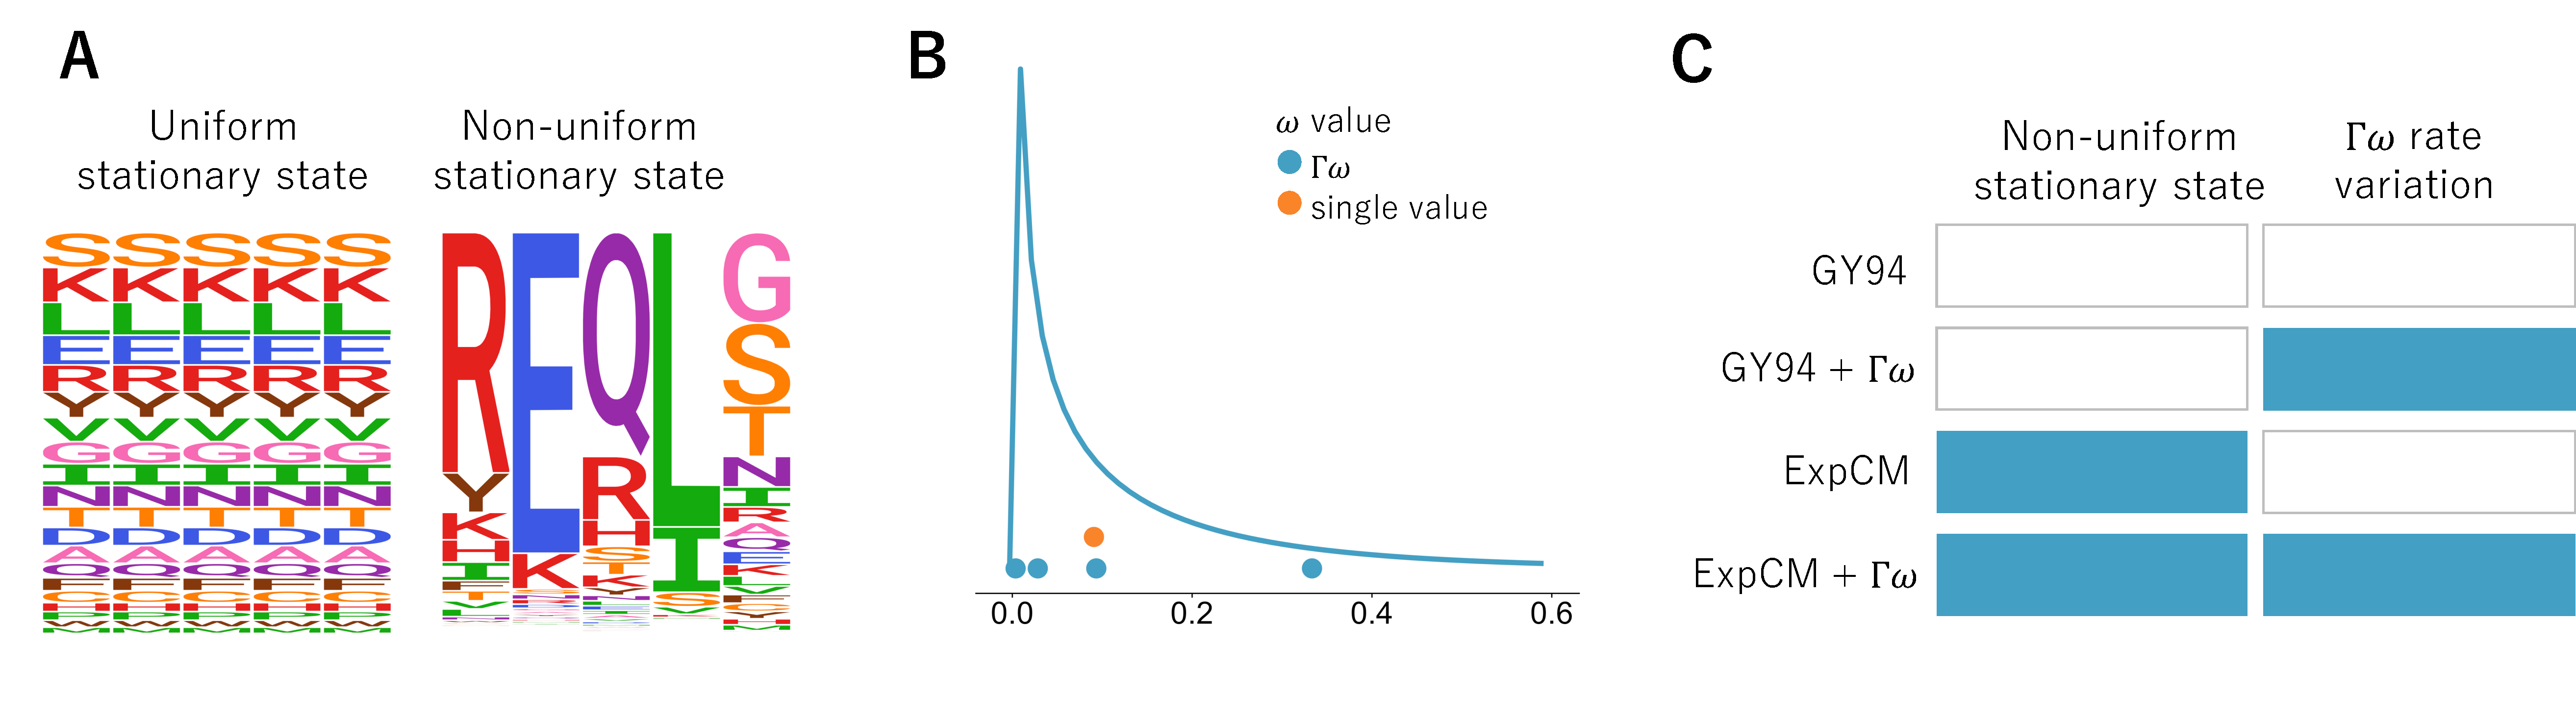
\includegraphics[width=0.90\textwidth]{figures/model_feature.pdf}}
\caption{\label{fig:model_feature}
\textbf{Different ways of modeling the site-to-site rate variation of purifying selection.}
(A) The dN/dS parameter, $\omega$, can be defined as one gene-wide average (orange triangle) or allowed to vary according to some statistical distribution (blue circles). 
In order to achieve computational tractability, the distribution is discretized into $K$ bins and $\omega$ takes on the mean of each bin. 
A gamma distribution ($\Gamma$) with $K=4$ bins is shown here.
(B) A substitution model stationary state defines the expected sequence composition after a very long evolutionary time. 
Most substitution models have stationary states that are uniform across sites.
However, substitution models can have site-specific stationary states.
In the logo plots, each column is a site in the protein and the height of each letter is the frequency of that amino acid at stationary state. 
(C) Substitution models can incorporate neither, one, or both of these features.
Here we will use substitution models from the \citet{goldman1994codon} (GY94) and experimentally informed codon model~\citep[ExpCM;][]{hilton2017phydms} families with and without gamma-distributed rates to represent all possible combinations. 
%Green indicates presence of a feature and white indicates absence. 
}
\end{figure}

Proteins evolve under purifying selection to maintain their structure and function. 
This purifying selection is not homogenous across sites in a protein.
It is also not homogenous among the different amino acids at a given site.
For instance, some protein sites strongly prefer hydrophobic amino acids, others may be constrained to just one or a few amino acids, and yet others may tolerate many amino acids.
In general, these constraints are highly idiosyncratic among sites, and so pose a challenge for phylogenetic substitution models.

Here we consider how purifying selection is handled by codon models, which are the most accurate of the three classes (nucleotide, amino acid, and nucleotide) of phylogenetic substitution models in widespread use~\citep{arenas2015trends}.
Codon models distinguish between two types of substitutions: synonymous and nonsynonymous.
The relative rate of these substitutions is referred to as dN/dS or $\omega$.
In their simplest form, codon substitution models fit a single $\omega$ that represents the gene-wide average selection on nonsynonymous mutations relative to synonymous ones.
Here we will use such substitution models in the form proposed by \citet{goldman1994codon}.
Using the classification scheme of \citet{yang2000codon}, when these models have a single gene-wide $\omega$ they are called M0.
We will refer to the M0 variant of the \citet{goldman1994codon} model simply as GY94.
The gene-wide $\omega$ is usually $<1$\citep{murrell2015gene}, and crudely represents the fact that many amino-acid substitutions are under purifying selection.

A single gene-wide $\omega$ ignores the fact that purifying selection is heterogeneous across sites.
The most common strategy to ameliorate this defect is to allow $\omega$ to vary among sites according to some statistical distribution~\citep{yang1994maximum,yang2000codon}.
For instance, in the M5 variant of the GY94 model~\citep{yang2000codon}, $\omega$ follows a gamma distribution as shown in \ref{fig:model_feature}A.
We will denote this model as GY94+$\Gamma\omega$.
A GY94+$\Gamma\omega$ captures the fact that the rate of nonsynonymous change can vary across sites. 
However, this formulation treats all nonsynonymous substitutions equivalently, since the rate is agnostic to the amino-acid identity of the mutation. 

A model formulation that accounts for the fact that purifying selection depends on the specific amino-acid mutation is provided by so-called ``mutation-selection'' models~\citep{halpern1998evolutionary,yang2008mutation,rodrigue2010mutation,tamuri2012estimating,mccandlish2014modeling}.
These models by explicitly define a different set of amino-acid preferences at each site in the protein. 
This more mechanistic formulation results in a site-specific stationary state (\ref{fig:model_feature}B). 
These models capture the site-to-site variation in amino-acid composition that is an obvious features of real proteins, and generally better describe actual evolution than models with only rate variation~\citep{lartillot2004bayesian, le2008phylogenetic, rodrigue2010mutation,hilton2017phydms,bloom2014experimentally}.

However, the increased realism of mutation-selection models comes at the cost of an increased number of parameters. 
Codon substitution models with uniform stationary states have only a modest number of parameters that must be fit from the phylogenetic data.
For instance, a GY94+$\Gamma\omega$ model with the commonly used F3X4 stationary state has 12 parameters: two describing the shape of the gamma distribution over $\omega$, a transition-transversion rate, and 9 parameters describing nucleotide composition of the stationary state.
However, mutation-selection models must additionally specify 19 parameters defining the stationary state for \emph{each} site (there are 20 amino acids whose frequencies are constrained to sum to one).
This corresponds to $19\times L$ parameters for a protein of length $L$, or 9500 parameters for a 500-residue protein.
It is challenging to obtain values for these parameters without overfitting the data~\citep{rodrigue2013statistical}.
Here we will primarily use experimentally informed codon models (ExpCM)~\citep{bloom2014experimentally, hilton2017phydms, bloom2017identification} which define values for these parameters \textit{a priori} from deep mutational scanning experiments~\citep{fowler2014deep} so they do not need to be fit from phylogenetic data.
Therefore, the number of remaining free parameters for an ExpCM are similar to a non-site-specific substitution model.
Alternative strategies of obtaining parameters for site-specific stationary states via Bayesian\skhcomment{cite} or maximum-likelihood estimation\skhcomment{cite} are discussed in the last section of the Results.

Importantly, these two strategies for modeling purifying selection are not mutually exclusive.
Mutation-selection models such as ExpCM can still incorporate an $\omega$ parameter, which now represents the relative rate of nonsynonymous to synonymous substitution \emph{after} accounting for the constraints due to the site-specific stationary state.
This $\omega$ parameter for an ExpCM can be drawn from a distribution just like for GY94-style models. 
We will denote such models as ExpCM+$\Gamma\omega$.
\ref{fig:model_feature}C shows the full spectrum of models that incorporate all combinations of gamma-distributed $\omega$ and site-specific stationary states.

\subsection*{Effect of stationary state and rate variation on branch-length estimation}

\begin{figure}
\centerline{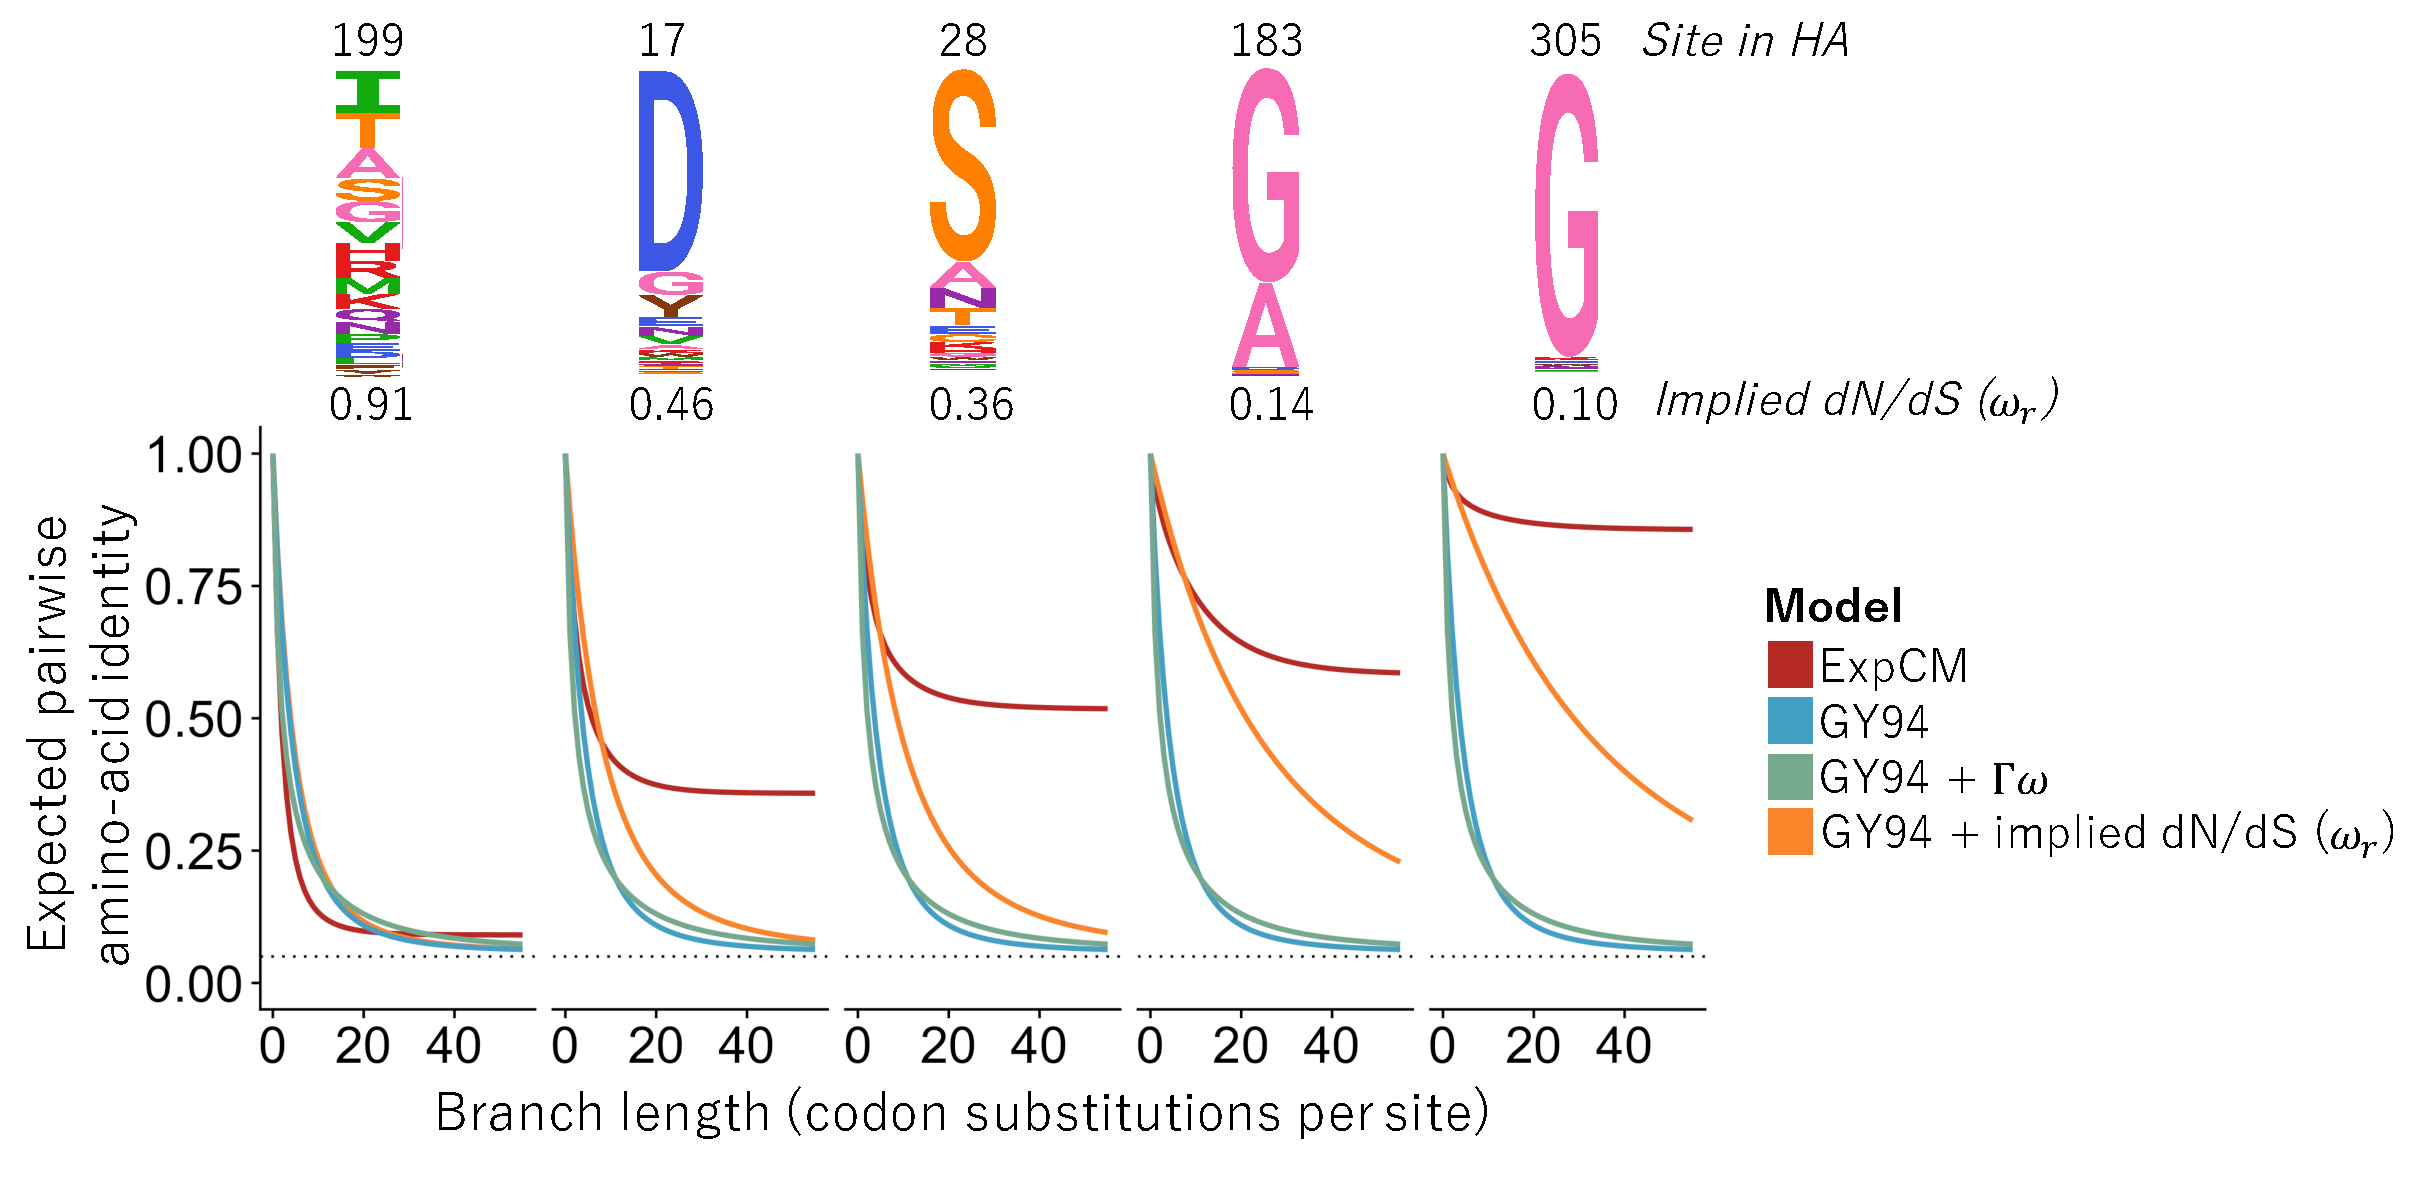
\includegraphics[width=0.90\textwidth]{figures/decay.pdf}}
\caption{\label{fig:decay}
\textbf{Effect of stationary state and $\Gamma\omega$ rate variation on predicted asymptotic sequence divergence.}
The logo plots at top show the amino-acid preferences for some sites in an H1 influenza hemagglutinin protein as measured by \citet{doud2016accurate}.
The graphs show the expected amino-acid identity at that site for two sequences separated by a branch of the indicated length (\ref{eq:f}).
For the GY94 model, the graphs are identical for all sites since this models does not have site-specific parameters; the same is true for GY94+$\Gamma\omega$.
The graphs do differ among sites if we use the amino-acid preferences to calculate a different $\omega_r$ value for each site $r$ in a GY94 framework~\citep[\ref{eq:w_r};][]{spielman2015relationship}.
However, all GY94 models including the one with site-specific $\omega_r$ values all approach the same asymptote since they all have the same stationary state.
But the ExpCM has different asymptotes for different sites since it accounts for how amino-acid preferences lead to site-specific stationary states.
}
\end{figure}

Given a single branch, a substitution model transforms sequence identity into branch length.
Under a molecular-clock assumption, this branch length is proportional to time.
The transformation from sequence identity to branch length is trivial when the sequence identity is high.
For instance, when where there has only been one substitution, then the sequence identity will simply be $\frac{L - 1}{L}$ for a gene of $L$ sites, and even a simple exponential model~\citep{zuckerkandl1965} will correctly infer the short branch length of $1/L$ substitutions per site.
However, as more substitutions accumulate then it becomes progressively more likely for multiple changes to occur at the same site.
In this regime, the accuracy of the substitution model becomes critical for transforming the sequence identity into branch length.
Any time-homogenous substitution model predicts that after a very large number of substitutions, two related sequences will approach some asymptotic sequence identity.
For instance, if all 20 amino acids are equally likely in the stationary state, then this asymptotic sequence identity will be 0.05.
If the substitution model underestimates the asymptotic sequence divergence then it will also underestimate long branch lengths, since it will predict that sequences that have evolved for a very long time should be more diverged than is actually the case.

\ref{fig:decay} shows how different substitution models predict sequence identity to decrease as a function of branch length for model parameters fit to a phylogeny of H1 influenza hemagglutinin (HA) genes.
The GY94 model predicts the same behavior for all sites, since it does not have any site-specific parameters.
This model predicts an asymptotic sequence divergence of \jdbcomment{?}, which is slightly higher than 0.05 since some of the 20 amino acids are favored due to more redundant codons and biases towards certain nucleotides.
Intuitively, this asymptotic sequence identity of \jdbcomment{?} seems low, since like many proteins HA has a highly conserved structure and function that imposes constraints that cause some sites to only sample a small subset of the 20 amino acids among all known HA homologs\jdbcomment{citation, I think Juhye has something she cites that looks at really diverged HAs}.

Accounting for site-to-site rate variation in GY94 models affects the rate at which the asymptotic sequence identity is approached, but not the actual value of this asymptote. 
For instance, \ref{fig:decay} shows that the GY94+$\Gamma\omega$ model takes longer to reach the asymptote than GY94, but the asymptote for both models is identical. 
This fact holds true even if we use experimental measurements of HA's site-specific amino-acid preferences~\citep{doud2016accurate} to calculate a different $\omega_r$ value for each site using the method of \citet{spielman2015relationship} (see \ref{eq:w_r}).
Specifically, this GY94+$\omega_r$ model predicts that different sites will approach the asymptote at different rates, but the asymptote is always the same (\ref{fig:decay}).
The invariance of the asymptotic sequence identity under different schemes for modeling $\omega$ is a fundamental feature of the mathematics of reversible substitution models.
These models are mathematically represented by reversible stochastic matrices, which can be decomposed into stationary states and symmetric exchangeability matrices~\citep{nielsen2006statistical}.
The stationary state is invariant with respect to multiplication of the symmetric exchangeability matrix by any non-zero number.
Different schemes for modeling $\omega$ only affect elements of the symmetric exchangeability matrix.
Therefore, no matter how ``well" a model accounts for site-to-site variation in $\omega$, it will always have the same stationary state as a simple GY94 model. 

However, mutation-selection models such as ExpCM's have site-specific stationary states.
Therefore, they predict that different sites will have different asymptotic sequence identities (\ref{fig:decay})---a prediction that accords with the empirical observation that some sites are much more variable than others in alignments of highly diverged sequences.
For instance, \ref{fig:decay} shows that at sites such as 348 and 305 in the H1 HA, an ExpCM but not a GY94-style model predicts that the divergence will always be low. 
When sites with highly constrained amino-acid preferences such as these are common, an ExpCM can estimate a very long branch length at modest sequence identities that GY94 model might attribute to a much shorter branch.


\subsection*{Simulations demonstrate how failure to model site-specific stationary states leads to branch-length underestimation.}
\begin{figure}
\centerline{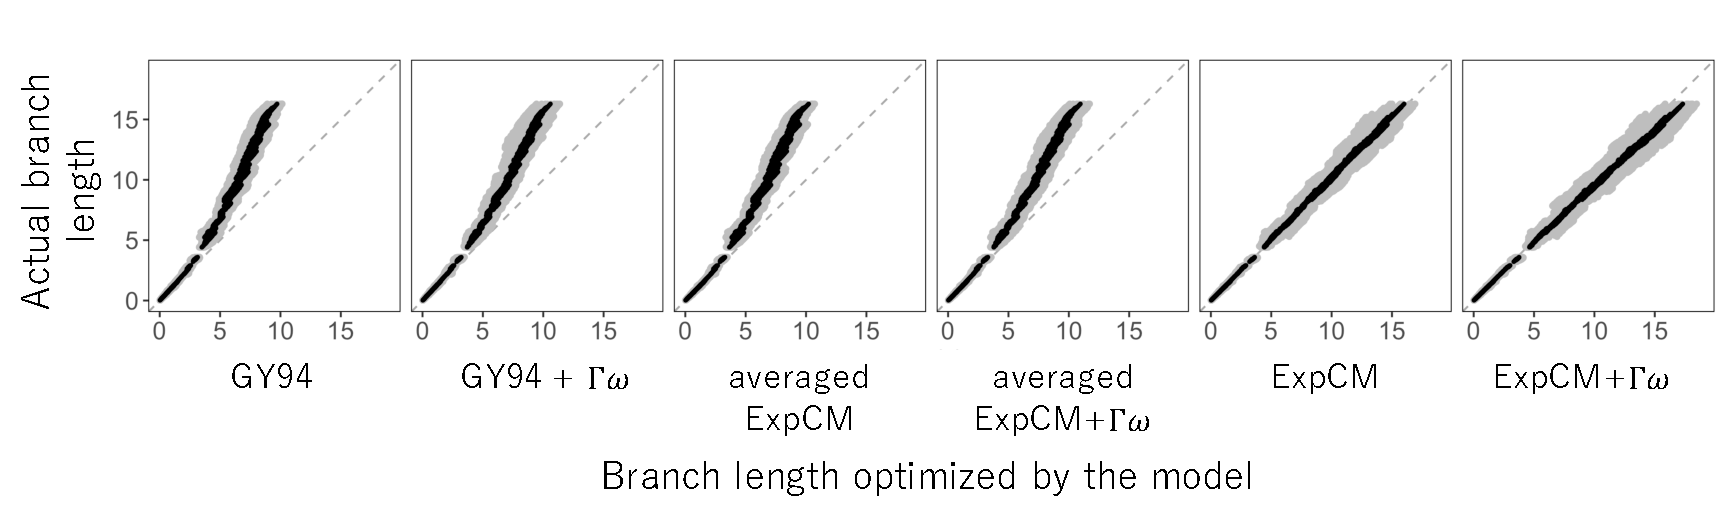
\includegraphics[width=0.85\textwidth]{figures/simulations}}
\caption{\label{fig:simulations}
\textbf{Branch lengths inferred on data simulated under a model with site-specific amino-acid preferences.} 
We simulated alignments along a phylogenetic tree of HA genes (see Figure~\ref{fig:empirical_trees}) using an ExpCM parameterized by the actual site-specific amino-acid preferences measured by deep mutational scanning of an H1 HA~\citep{doud2016accurate}.
We then inferred the branch lengths of this tree on the simulated alignments.
The inferred branch lengths for various models are plotted on the x-axis, and the actual branch lengths used in the simulations are on the y-axis.
We performed 10 simulations and inferences, and gray points show each inferred branch length from each simulation, and black points show the average of each branch length across simulations.
The grey dashed line at $y=x$ represents the behavior of an unbiased estimator. 
}
\end{figure}
To directly demonstrate the effect of stationary state and $\Gamma\omega$ rate variation on branch-length estimation, we tested the ability of a variety of models to accurately infer branch lengths on simulated data (\ref{fig:simulations}).
Specifically, we simulated alignments of sequences along the HA phylogenetic tree in \ref{fig:empirical_trees}) using ExpCM parameterized by the actual amino-acid preferences of H1 HA as experimentally measured by deep mutational scanning~\citep{doud2016accurate}. We then estimated the branch lengths from the simulated sequences using all the substitution models in \ref{fig:model_feature}C, and compared these estimates to the actual branch lengths used in the simulations.

The models with a uniform stationary state underestimated the lengths of long branches separating the simulated sequences (\ref{fig:simulations}). 
The GY94 model estimated branches lengths which are only about 60\% of the true values for the longest branches. 
Accounting for site-to-site variation in $\omega$ did not fix the fundament problem: the GY94+$\Gamma\omega$ did slightly better, but still substantially underestimated the length of the longest branches.
However, there was no systematic underestimation of long branches by the ExpCM and ExpCM+$\Gamma\omega$ models, which accurately accounted for the site-specific amino-acid preferences used in the simulations.
The improved performance of the ExpCM's is due to their site-specific modeling of the stationary state: if we parameterize these models by site-specific amino-acid preferences that have been averaged across HA sites, then they perform no better than GY94 models.
Therefore, models with uniform stationary states are fundamentally incapable of accurately estimating the length of long branches in phylogenies of sequences that have evolved under strong site-specific amino-acid preferences.


\subsection*{Site-specific models estimate longer branches on real data.}

\begin{figure}
\centerline{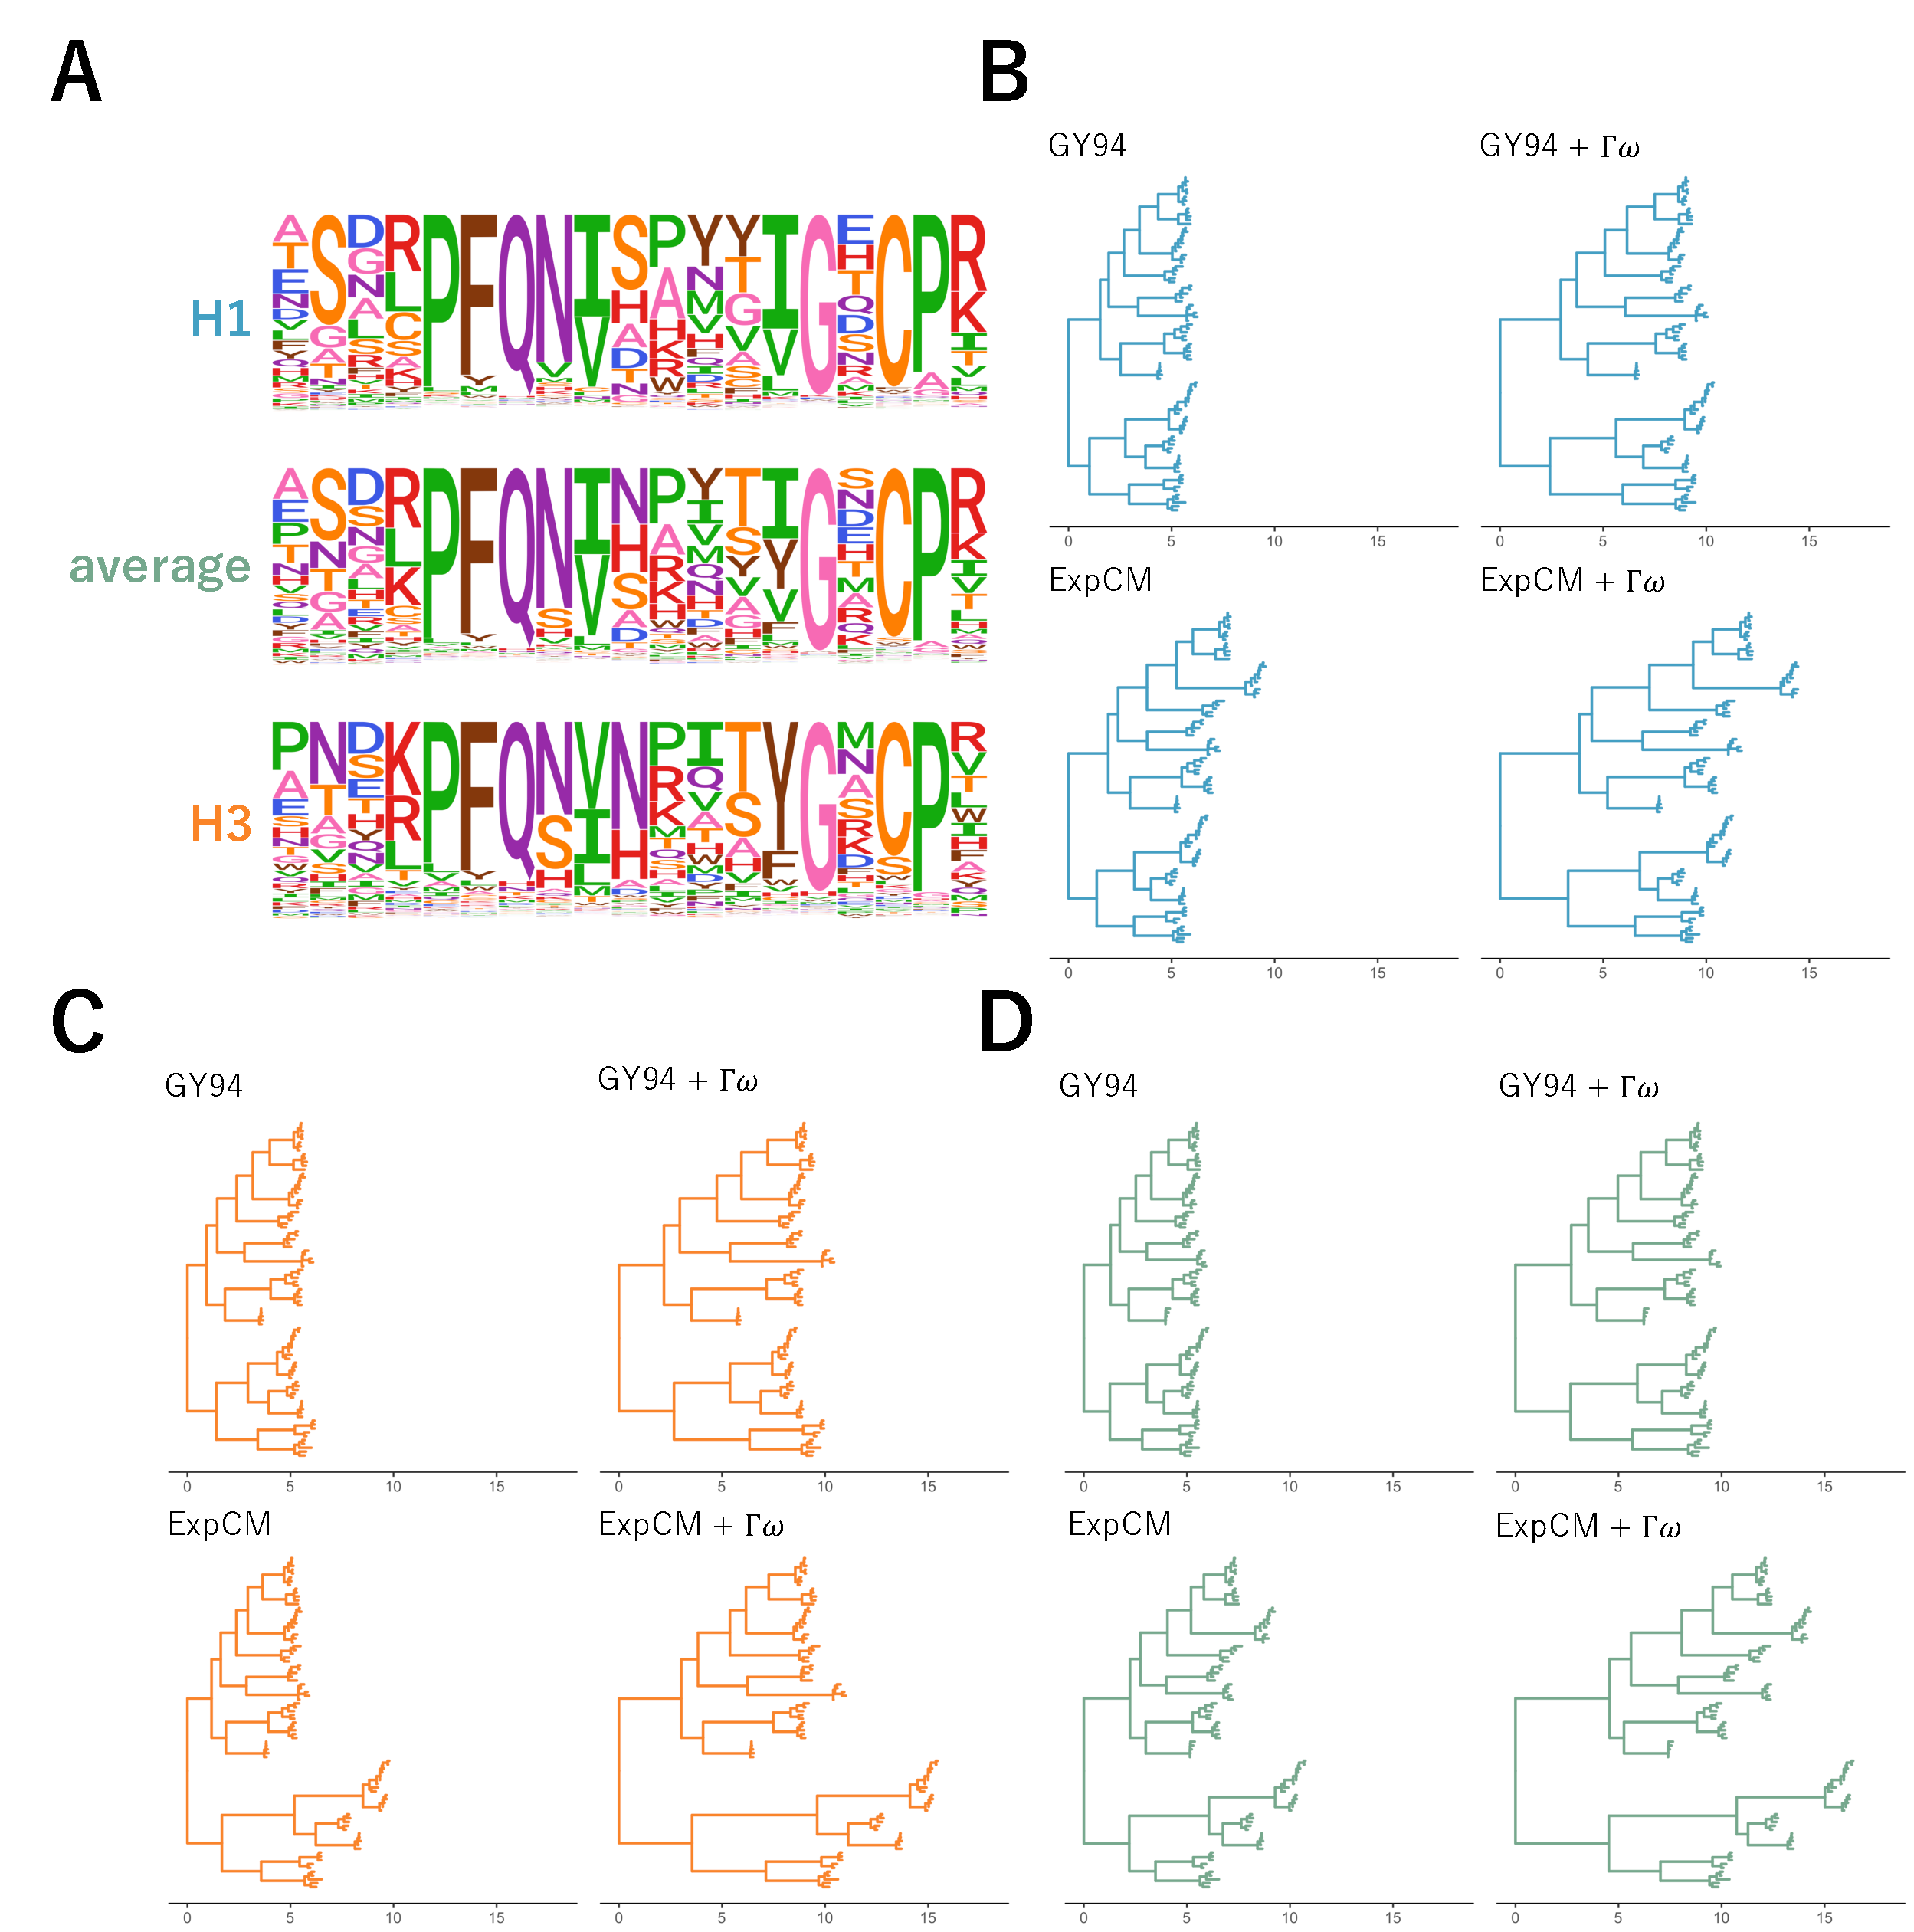
\includegraphics[width=\textwidth]{figures/empirical_trees.pdf}}
\caption{\label{fig:empirical_trees}
\textbf{Effect of site-specific stationary state and $\Gamma\omega$ rate variation on HA branch length estimation.} 
The HA tree is optimized by models from the ExpCM and GY94 families. 
The amino-acid preferences defining the model (ExpCM) or implied by the model (GY94) are shown as logoplots. 
The amino-acid preferences measured by the deep mutational scans defining the ExpCMs were measured in either an H1 background, an H3 background, or were the average measurements from the H1 and H3 scans. 
The circle denotes the H1 clade and the triangle denotes the H3 clade. 
}
\end{figure}

\begin{table}[t!]
\caption{\label{tab:empirical_data}
Performance comparison for the models in~\ref{fig:empirical_trees}. 
All ExpCMs describe the evolution of HA better than the GY94 models, as evaluated by the Akaike information criteria~\citep[$\Delta$AIC,][]{posada2004model}
The mean $\omega$ value from each $K=4$ bins is shown for the models with $\Gamma\omega$ rate variation, otherwise simply the fit, gene-wide $\omega$. 
Each ExpCM has a stringency parameter $>1$.
} 
     \begin{tabular}{cccccccccc}
        \hline
         Model & $\Delta$AIC & {\shortstack{Log\\ Likelihood}} & {\shortstack{$\omega$\\ (implied dN/dS)}} & {\shortstack{stringency\\ parameter}}\\ \hline
       	ExpCM + $\Gamma\omega$ (H1+H3 avg)  & 0 & -48751 & 0.19,  0.50,  0.90,  1.86 &  1.70\\
	ExpCM (H1+H3 avg)  &  950 & -49227 & 0.15 & 1.78\\
	ExpCM + $\Gamma\omega$ (H1)  & 1306 & -49404  & 0.13 ,  0.44,  0.91,  2.16 & 1.12\\
	ExpCM + $\Gamma\omega$ (H3) & 1737 & -49620 & 0.09,  0.33,  0.72,  1.77 & 1.28\\
	ExpCM (H1) & 2556 & -50030 &  0.13 & 1.22\\
	ExpCM (H3) &  3197 & -50350 & 0.12 & 1.45\\
	GY94 + $\Gamma\omega$  & 4719 & -51106 & 0.00,  0.03,  0.08,  0.26 & - \\
	GY94 & 7625 & -52560  & 0.07 & -\\
      \end{tabular}
\end{table}

The foregoing section shows the superiority of ExpCM's to GY94 models for estimating long branches on phylogenies simulated with ExpCM models.
But how do these models perform on real rather than simulated data?
Real genes do evolve under site-specific constraint, but this constraint is almost certainly not modeled in all its complexity by an ExpCM.
However, if ExpCM's do a substantially better job of modeling the constraint, we might still expect them to estimate more accurate branch lengths.

To test the models on real data, we used actual sequences of influenza HA. 
The topology of HA phylogenetic trees (\ref{fig:empirical_trees}) makes these sequences an interesting test case for branch-length estimation.
HA consists of a number of different subtypes.
Sequences within a subtype have \jdbcomment{?} amino-acid identity, but sequences in different subtypes have as little as 38\% identity.
However, HA proteins from all subtypes (with the exception of an unusual subtype of bat influenza virus that we exclude from this analysis~\jdbcomment{?}) have a highly conserved structure that performs a highly conserved function\jdbcomment{citation, Juhye can probably help}.
We used \texttt{RAxML} with nucleotide model of substitution (GTRCAT) to infer a phylogenetic tree for 87 HA sequences drawn from 14 of the 18 subtypes (we excluded bat influenza and three other rare subtypes).
For the rest of this paper, we fix the tree topology to this \texttt{RAxML}-inferred tree.
Although the nucleotide model used with \texttt{RAxML} is probably less accurate than codon models, the modular subtype structure of the HA phylogeny means that most of the phylogenetic uncertainty probably lies in the length of the long branches separating the subtypes rather than in the tree topology itself.
 
Given this fixed HA tree topology, we estimated the branch lengths on the tree using each of the substitution models in \ref{fig:model_feature}C. 
There are two all amino-acid deep mutational scanning datasets for HA~\jdbcomment{citations}, and each parameterizes a different ExpCM.
One scan measured the site-specific amino-acid preferences in an H1 background (\ref{fig:empirical_trees}, circle) and the other measured the preferences in an H3 background (\ref{fig:empirical_trees}, triangle). 
These two deep mutational scans sample the breadth of HA diversity as their respective focal sequences are only $\sim42\%$ identical on the amino acid level. 
By comparing these two ExpCMs, we can examine the effect of the experiment's focal sequence on branch length estimation, along with the effect of site-specific stationary state and $\Gamma\omega$ rate variation.

The results in \ref{fig:empirical_trees} show the distinct effects of modeling variation in $\omega$ and variation in the stationary state. 
For two models with the same stationary state, the model which allows $\omega$ to vary estimates longer branches. 
For example, the GY94+$\Gamma\omega$ estimates longer branches on the HA tree than the GY94 and the ExpCM+$\Gamma\omega$(H1 prefs) estimates longer branches than the ExpCM(H1 prefs).
In addition, the models with site-specific stationary states estimate longer branches than the models with a uniform stationary state given the same $\omega$ parametrization.  
Both the ExpCM(H1 prefs) and ExpCM(H3 prefs) estimate longer branches than the GY94 model. 

However, in contrast to the effect of adding $\Gamma\omega$ rate variation, the effect of the site-specific stationary state defined by deep mutational scanning preferences in not uniform across the entire tree. 
The effect is largest on the branches near the focal sequence of the deep mutational scan for both the ExpCM(H1 prefs) and ExpCM (H3 prefs). 
While the ExpCM's show an increase in branch length with a strong local effect, the increase is seen even in the presence of $\Gamma\omega$ rate variation. 
The ExpCM+$\Gamma\omega$ estimates the longest branches for all of the models tested. 
These results indicate that the site-specificity of the ExpCM stationary state is important for long branch underestimation but this stationary state is not constant across the entire HA tree. 

\subsection*{Competing effects of shifting preferences and long branches.}

\begin{figure}[H]
\centerline{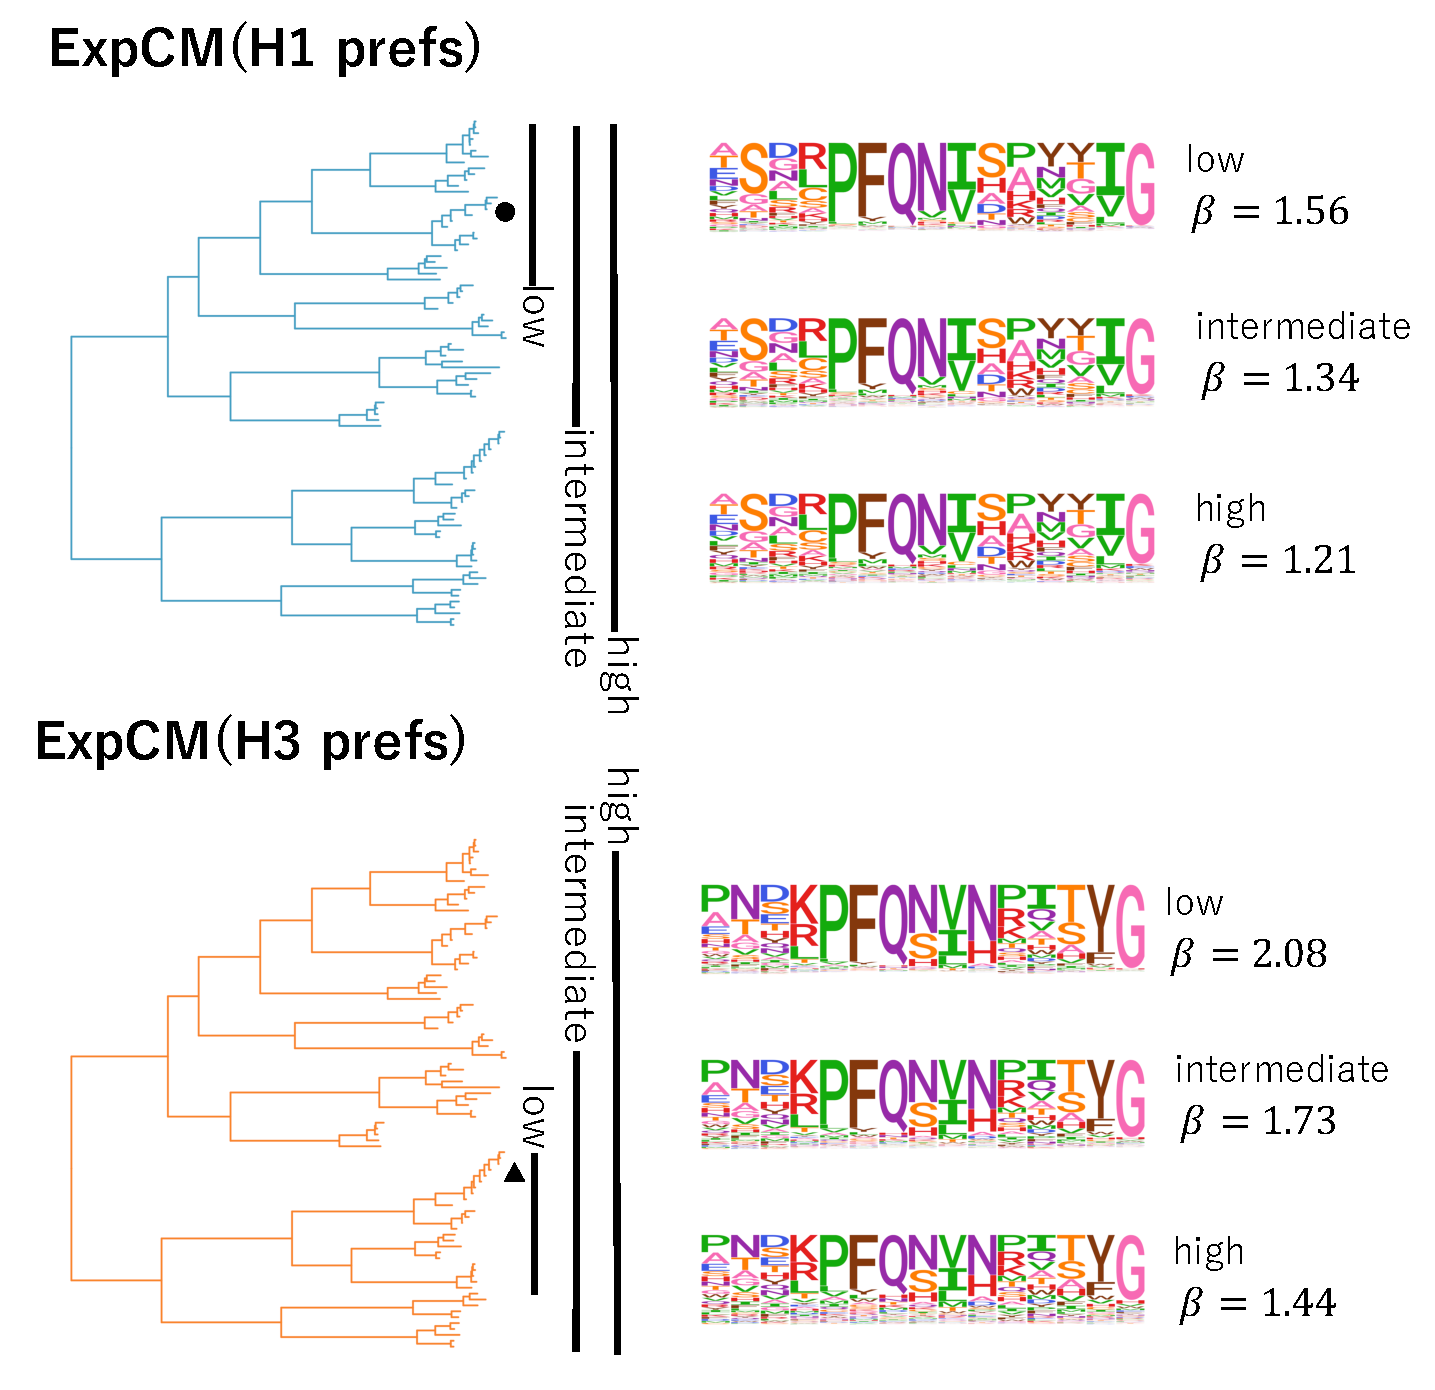
\includegraphics[width=0.85\textwidth]{figures/compete_3}}
\caption{\label{fig:compete}
\textbf{Effect of overall divergence on the congruency between natural sequences and the deep mutational scanning preferences.} 
For each deep mutational scanning preference set, we fit an ExpCM to three trees representing high, intermediate, and low overall divergence from the experimental focal sequence. 
We used the ExpCM stringency parameter ($\beta$) to determine the congruency between the natural sequences and the experimental measurements. 
A $\beta >1$ indicates that the natural sequences favor the same amino-acid preferences as the experimental measurements but with a greater strength. 
A $\beta < 1$ indicates the natural sequences do not favor the same amino-acid preferences as the experimental measurements or favor the same amino acids but less strongly. 
As the overall divergence increased, the $\beta$ value for the ExpCM(H3 prefs) and ExpCM(H1 prefs) decreased, indicating that the preferences do ``shift" over the full HA tree. 
\skhcomment{1. I need to clean up and do a better job aligning the different parts of this figure but what do you think of the overall layout? 2. \ref{supp:compete_4} shows an alternative layout.}
}
\end{figure}

The local effect of the ExpCM is not entirely surprising. 
Proteins are affected epistatic interactions, where the effect of a mutation at one site is dependent on the amino-acid identity at another site. 
While one of the strengths of deep mutational scanning is the ability to accurately measure the effect of all single amino-acid mutations, these measurements are done in the context of a single genetic background and do not take into account epistatic interactions. 
The stationary state of the ExpCM's is only as accurate as deep mutational scanning preferences and the results in \ref{fig:empirical_trees} indicate that any given deep mutational scan is most accurate for only a subset of the tree with closely related sequences to the focal sequence.  

%An ExpCM with a more general stationary state, defined by the average of the H1 and H3 preferences, increases the estimates of branch length from both the H1 and H3 clade (\ref{fig:empirical_trees}). 

We examined how the deep mutational scanning preferences shift across the full HA tree by comparing the ExpCM behavior on trees with varying levels of overall divergence from the ExpCM focal sequence. 
For each of the subtrees in \ref{fig:compete}, we asked "how well do the deep mutational scanning preferences agree with the natural sequences?" using the ExpCM stringency parameter $\beta$ (\ref{eq:Frxy}). 
The fit $\beta$ parameter rescales the raw preferences from the deep mutational scan and relates the selection in nature to selection in the lab. 
We interpret $\beta >1$ as selection in nature favoring the same amino acids as selection in the experiments, or that the amino-acid preferences are a good model of purifying selection. 
The larger the $\beta$ more strongly the selection in nature favors these same, experimental preferences. 
Conversely, we interpret a $\beta<1$ as selection in nature favoring different amino acids than selection in lab and that the preferences are not a good description of natural evolution.  
\skhcomment{mention pop-gen derivation and the relationship between lab vs. nature selection and pop size?}

The results in \ref{fig:compete} show that as the overall divergence from the focal sequence of a deep mutational scan increase, the $\beta$ value decreases. 
This inverse relationship between $\beta$ and overall divergence is seen for both the ExpCM(H1 prefs) and ExpCM(H3 prefs). 
Along with the local effect in branch length extension seen \ref{fig:empirical_trees}, this indicates that the amino-acid preferences have shifted across the HA tree. 
This leaves us in a regime with inherent tension. 
Models which take into account the site-specific constraints of purifying selection in their stationary states are important for the accurate estimation of long branches but the site-specific constraints are not static throughout evolution. 
Models with a single stationary state regardless of lineage, site-specific or not, will not be able to capture the shifting functional constraints due to epistatic interactions. 
\skhcomment{All betas are greater than 1 so the preferences are ``better" than the GY94 model even at high overall divergence.}

\subsection*{\texttt{phylobayes}}

The previous sections show that the ExpCM's, with their site-specific stationary states, estimate longer branches than the GY94. 
However, the ExpCM stationary state has a strong local effect as the amino-acid preferences from deep mutational scanning experiments are most accurate near their focal sequence. 
There are other models with site-specific stationary states which infer all of the parameters from the phylogenetic data rather than from independent experiments. 
For example, the CAT model, an amino-acid rather than codon model, describes the stationary state at each site as a mixture model of distinct, finite amino-acid profiles and the mutation-selection model implemented in \texttt{phylobayes} is almost identical to the ExpCM except the amino-acid preferences are inferred in a Bayesian framework rather than defined by deep mutational scanning experiments. 
We compared the ExpCM with the \texttt{phylobayes} mutation-selection model to examine the effect of site-specific stationary states on branch length estimation with and without experimental preferences. 

The results in \ref{fig:phylobayes} show that the ExpCM+$\Gamma\omega$(H1+H3 avg prefs) and the \texttt{phylobayes} mutation-selection model, which includes $\Gamma\omega$, estimated similar branch lengths on the HA tree in \ref{fig:empirical_trees}. 
While the two models estimated the same branch length on average, the tension between local and global accuracy is still apparent in the results. 
All of the long branches from either the H1 or H3 focal sequence were estimated to be longer by the ExpCM+$\Gamma\omega$ while all other branches were estimated to be longer by the \texttt{phylobayes} mutation-selection model. 
This enrichment of branches from the focal sequence in the branches estimated to be longer by the ExpCM+$\Gamma\omega$(H1+H3 prefs) indicates that the ``global" stationary state inferred by \texttt{phylobayes} is not as accurate as the deep mutational scanning preferences for sequences close to the focal sequence. 
The accuracy of the deep mutational scanning preferences is sacrificed for more a universal stationary state. 
While the parameters inferred by the \texttt{phylobayes} model are a good compromise, they do not avoid the tension between the importance of a site-specific stationary state for long branch estimation and shifting preferences. 


\begin{figure}[H]
\centerline{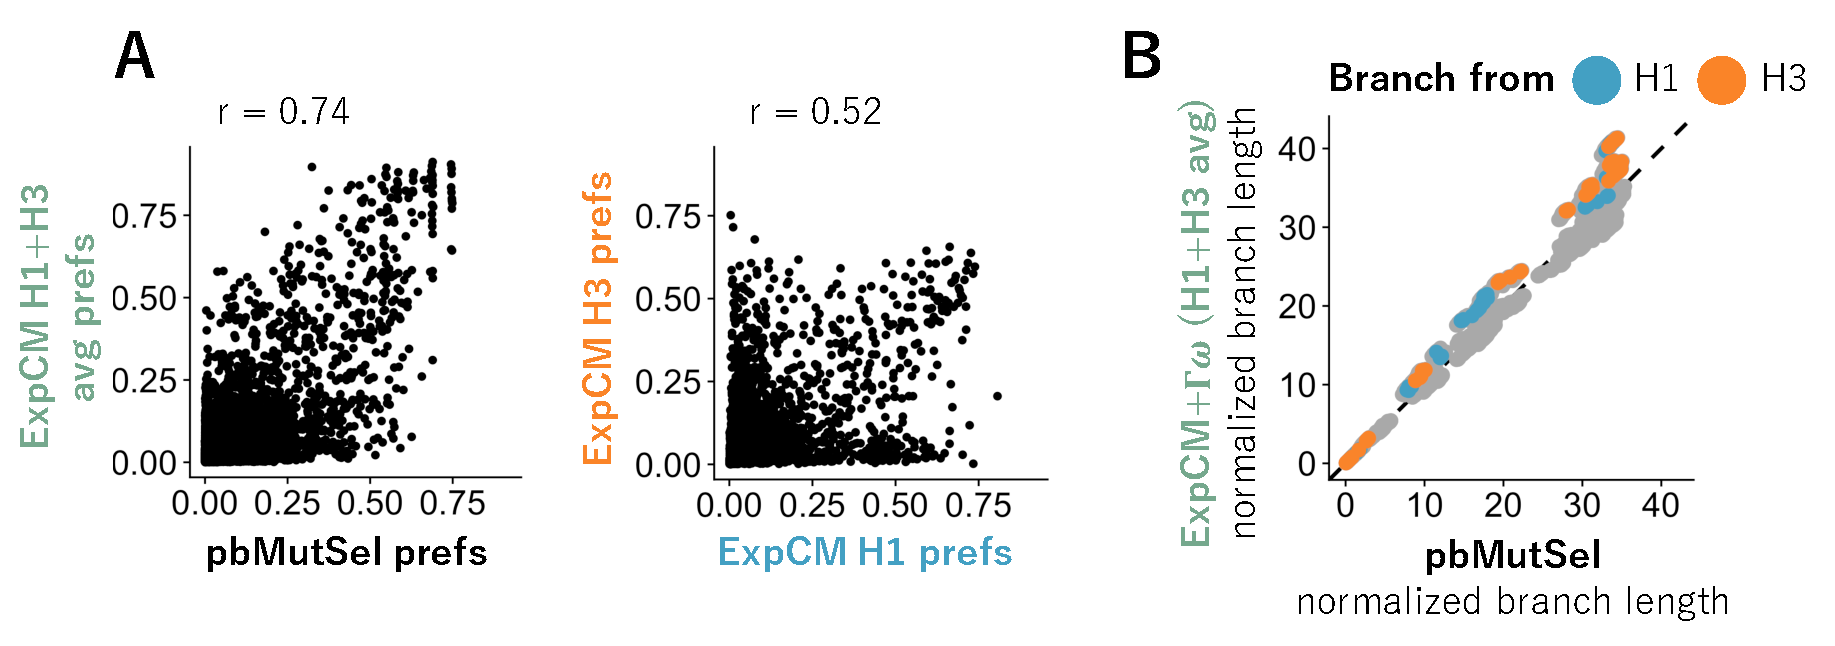
\includegraphics[width=0.5\textwidth]{figures/phylobayes.pdf}}
\caption{\label{fig:phylobayes}
\textbf{Comparison of ExpCM and \texttt{phylobayes}}
We estimated the branch lengths of the HA tree in \ref{fig:empirical_trees} using the mutation-selection model implemented in \texttt{phylobayes}. 
In comparison to ExpCM's, the \texttt{phylobayes} model infers the site-specific amino-acid preferences from the phylogenetic data rather than defining them \textit{a priori} from deep mutational scanning experiments. 
}
\end{figure}

\section*{Conclusion}

\begin{enumerate}
  \item We don't allow any of the models to vary by lineage. 
\end{enumerate}

\newpage
\section*{Materials and Methods}

\subsection*{Substitution models}
\subsubsection*{GY94 models}
\subsubsection*{ExpCMs}
We recap the \textbf{Exp}erimentally Informed \textbf{C}odon \textbf{M}odel (ExpCM) \citep{bloom2014experimentally,bloom2014informed,bloom2017identification,hilton2017phydms} to introduce nomenclature. 

In an ExpCM, rate of substitution $P_{r,xy}$ of site $r$ from codon $x$ to $y$ is written in mutation-selection form~\citep{halpern1998evolutionary,mccandlish2014modeling,spielman2015relationship} as
\begin{equation}
P_{r,xy} = Q_{xy} \times F_{r,xy}
\end{equation}
where $Q_{xy}$ is proportional to the rate of mutation from $x$ to $y$, and $F_{r,xy}$ is proportional to the probability that this mutation fixes.
The rate of mutation $Q_{xy}$ is assumed to be uniform across sites, and takes an HKY85-like~\citep{hasegawa1985dating} form:
\begin{equation}
Q_{xy} = 
\begin{cases}
\phi_w & \mbox{if $x$ and $y$ differ by a transversion to nucleotide $w$} \\
\kappa \phi_w & \mbox{if $x$ and $y$ differ by a transition to nucleotide $w$} \\
0 & \mbox{if $x$ and $y$ differ by $>1$ nucleotide.}
\end{cases}
\end{equation}
The $\kappa$ parameter represents the transition-transversion ratio, and the $\phi_w$ values give the expected frequency of nucleotide $w$ in the absence of selection on amino-acid substitutions, and are constrained by $1 = \sum_w \phi_w$.

The deep mutational scanning data are incorporated into the ExpCM via the $F_{r,xy}$ terms.
The experiments measure the preference $\pi_{r,a}$ of every site $r$ for every amino-acid $a$.
The $F_{r,xy}$ terms are defined in terms of these experimentally measured amino-acid preferences as
\begin{equation}
\label{eq:Frxy}
F_{r,xy} = 
\begin{cases}
   1 & \mbox{if $\mathcal{A}\left(x\right) = \mathcal{A}\left(y\right)$} \\
   \omega \times \frac{\ln\left[\left(\pi_{r,\mathcal{A}\left(y\right)} / \pi_{r,\mathcal{A}\left(x\right)}\right)^{\beta}\right]}{1 - \left(\pi_{r,\mathcal{A}\left(x\right)} / \pi_{r,\mathcal{A}\left(y\right)}\right)^{\beta}} & \mbox{if $\mathcal{A}\left(x\right) \ne \mathcal{A}\left(y\right)$}
   \end{cases}
\end{equation}
where $\mathcal{A}\left(x\right)$ is the amino-acid encoded by codon $x$, $\beta$ is the stringency parameter, and $\omega$ is the relative rate of nonsynonymous to synonymous substitutions after accounting for the amino-acid preferences.
The ExpCM has six free parameters (three $\phi_w$ values, $\kappa$, $\beta$, and $\omega$).
The preferences $\pi_{r,a}$ are \emph{not} free parameters since they are determined by an experiment independent of the sequence alignment being analyzed.

The ExpCM stationary state frequency $p_{r,x}$ of codon $x$ at site $r$ is~\citep{bloom2017identification} 
\begin{equation}
\label{eq:p_rx}
p_{r,x} = \frac{\left(\pi_{r,\mathcal{A}\left(x\right)}\right)^{\beta} \phi_{x_0} \phi_{x_1} \phi_{x_2}}{\sum_z \left(\pi_{r,\mathcal{A}\left(z\right)}\right)^{\beta} \phi_{z_0} \phi_{z_1} \phi_{z_2}},
\end{equation}
\subsection*{Theoretical effect of model choice on branch length}
\subsection*{Effect of model choice on natural sequences}

\subsubsection*{ExpCM + $\Gamma\omega$ and YNGKP M5}


\subsubsection*{Spielman $\omega_{r}$ values inferred from the ExpCM} 
We inferred the average nonsynonymous fixation rate from the ExpCM following~\citet{spielman2015relationship} as 
\begin{equation}
\label{eq:w_r}
\omega_{r} = \frac{\sum_{x} \sum_{y \in N_x} {p_{r,x} \times P_{r,xy}}}{\sum_{x} \sum_{y \in N_x} {p_{r,x} \times Q_{xy}}}
\end{equation}
where $p_{r,x}$ is the stationary state of the ExpCM at site $r$ and codon $x$, $P_{r,xy}$ is the substitution rate from codon $x$ to codon $y$ at site $r$, $Q_{xy}$ is the mutation rate from codon $x$ to codon $y$, and $N_x$ is the set of codons that are nonsynonymous to codon $x$ and differ from codon $x$ by only one nucleotide. 

\subsubsection*{Expected pairwise amino-acid identity}
\textit{Do I need to talk about the branchScale scaling I used?}
The expected pairwise amino-acid identity at a site $r$ over time $t$ for a given model is 
\begin{equation}
\label{eq:f}
\sum_a \sum_{x \in a} p_{r,x} \sum_{y \in a} [M_{r}\left(t\right)]_{xy}
\end{equation}
where $a$ is all amino acids, $p_{r,x}$ is the stationary state of the model at site $r$ and codon $x$, and $[M_{r}\left(t\right)]_{xy}$ is the transition rate from codon $x$ to codon $y$ at site $r$ given time $t$. 

\newpage
\section*{Supplemental Information}

\subsection*{Model Parameters for the simulations}

\begin{suppfig}[H]
\centerline{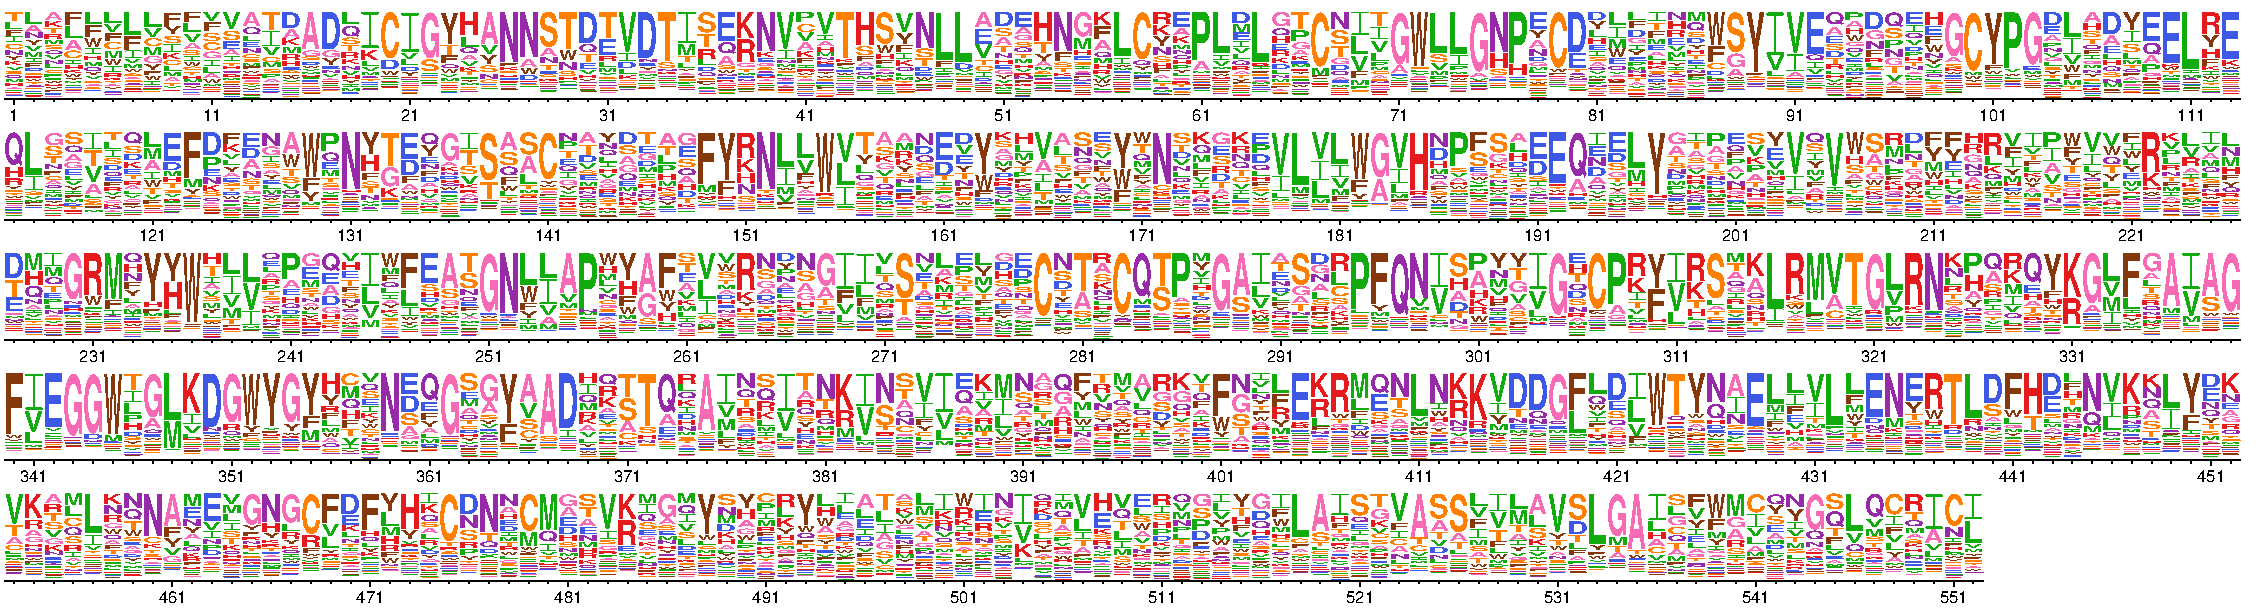
\includegraphics[width=\textwidth]{figures/prefs_doud}}
\caption{\label{suppfig:prefs_doud}
\textbf{H1 preferences measured by \cite{doud2016accurate} rescaled with the ExpCM stringency parameter optimized in \ref{fig:tree_doud}A  ($\beta = 1.19$)} 
\skhcomment{I need to change the $\beta$ value when the new \texttt{phydms} results finish running.}
}
\end{suppfig}

\begin{suppfig}[H]
\centerline{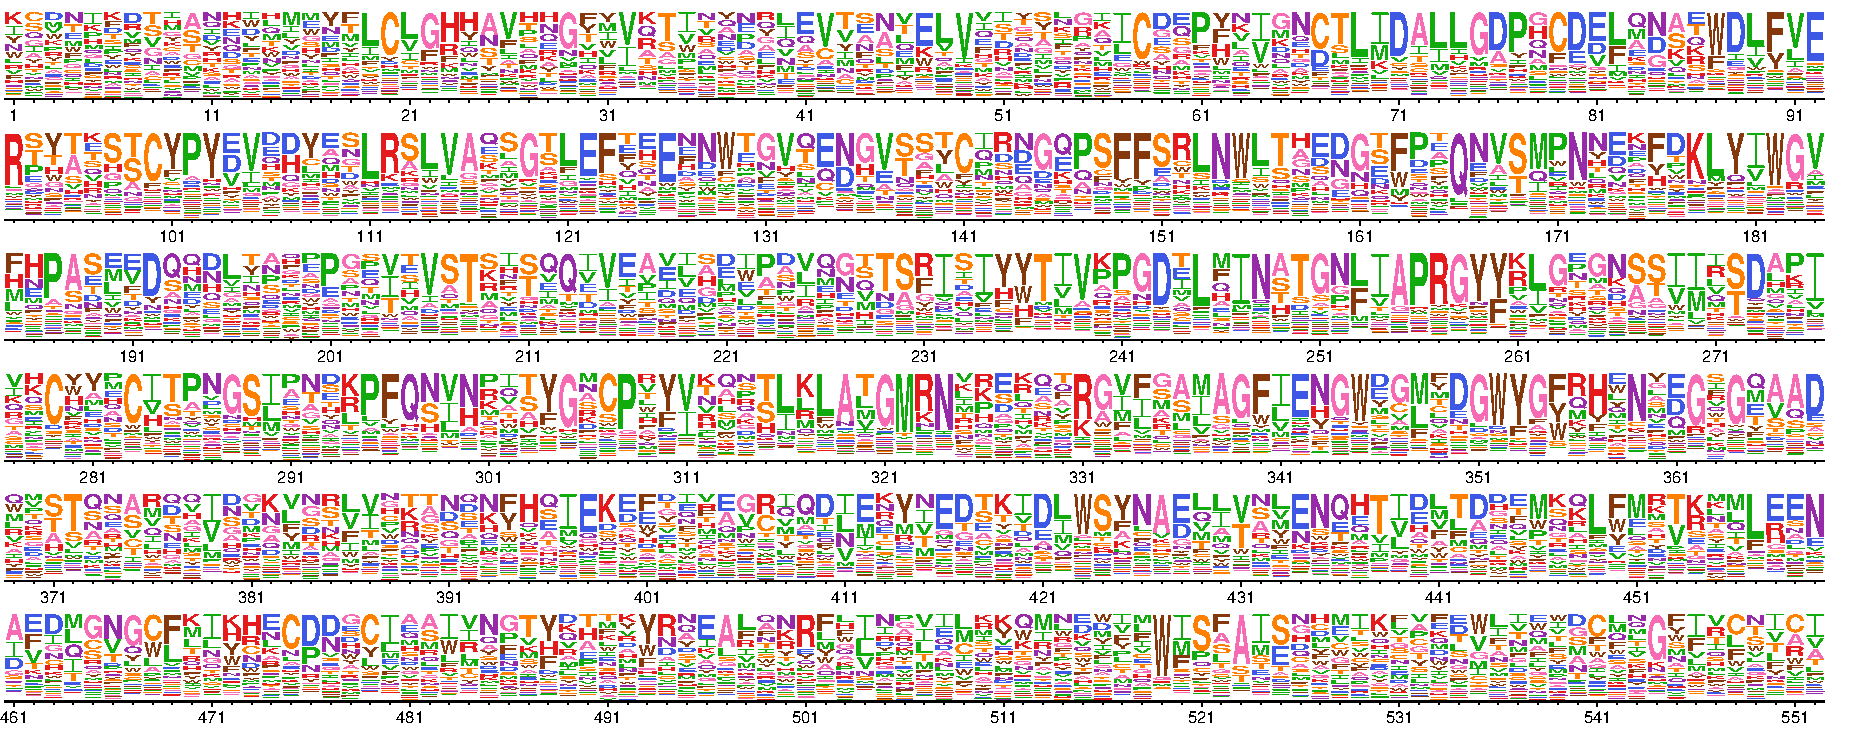
\includegraphics[width=\textwidth]{figures/prefs_lee}}
\caption{\label{suppfig:prefs_lee}
\textbf{H3 preferences measured by \textit{lee} rescaled with the ExpCM stringency parameter optimized in \ref{fig:tree_lee}A  ($\beta = 1.46$)}
 }
\end{suppfig}

\begin{suppfig}[H]
\centerline{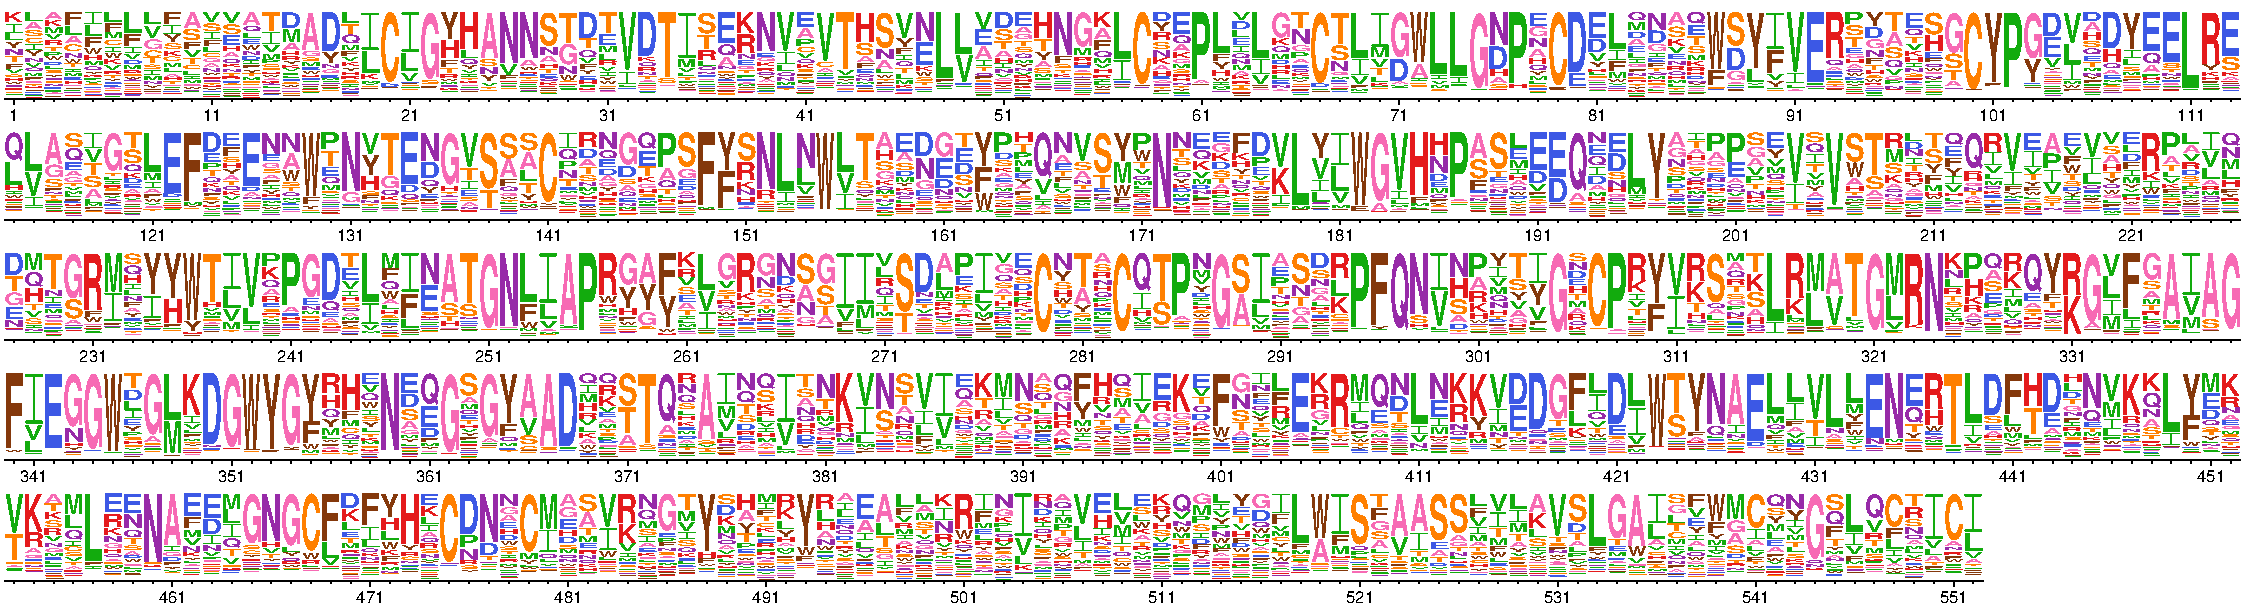
\includegraphics[width=\textwidth]{figures/prefs_average}}
\caption{\label{fig:prefs_average}
\textbf{The average of the H1 preferences measured by \cite{doud2016accurate} and the H3 preferences measured by \textit{Lee} rescaled with the ExpCM stringency parameter optimized in \ref{fig:tree_average}A  ($\beta = 1.77$)}}
\end{suppfig}
 

\begin{suppfig}[H]
\centerline{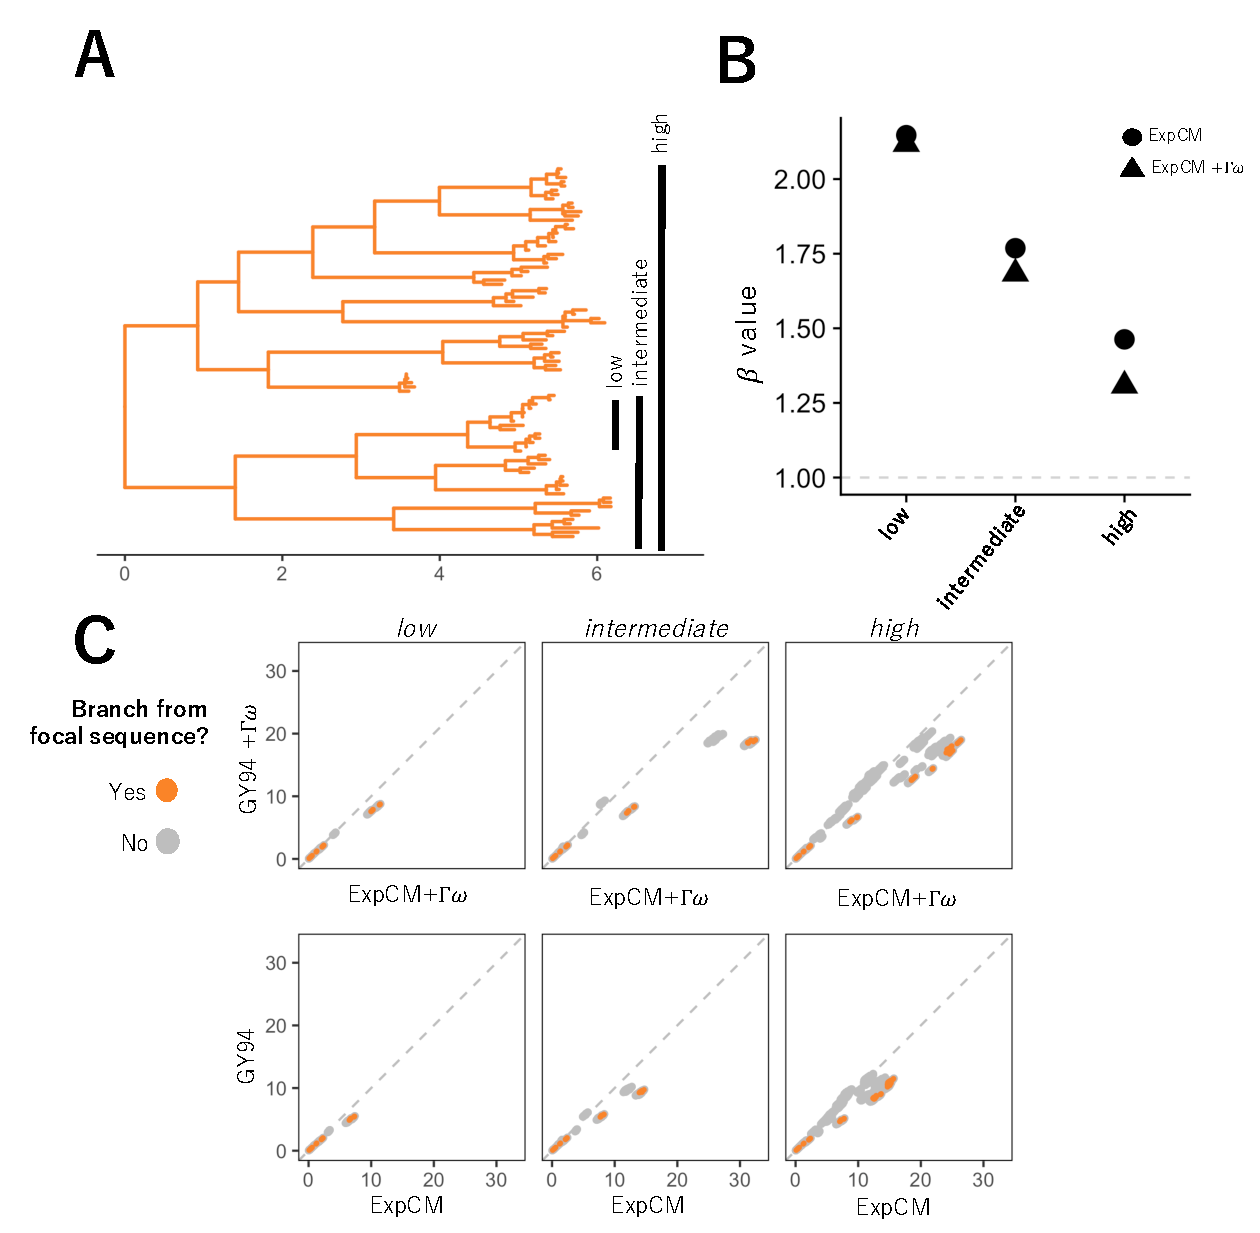
\includegraphics[width=0.85\textwidth]{figures/lee_compete}}
\caption{\label{supp:lee_compete}
\textbf{The ExpCM defined by H1 preferences lengthen longer branches on the HA tree.} 
\textbf{(A)} An HA alignment was subsampled to create three smaller alignments with varying degrees of divergence from the focal H3 sequence, referred to as "low", "intermediate", and "high". 
\textbf{(B)} The phylogenetic tree of the "high" alignment. 
The colors denote the alignment and the black circle denotes the focal H3 sequence. 
\textbf{(C)} The value of the ExpCM and ExpCM+$\Gamma\omega$ stringency parameter $\beta$ decreases as the divergence from the focal H3 sequence increases. 
\textbf{(D)} Comparisons of branch lengths optimized by the four substitution models for the varying degrees of divergence. 
Black points represent branches from the focal H3 sequence and grey points represent all other branches.  
The branch lengths are in average number of codon substitutions per site. 
}
\end{suppfig}

\begin{suppfig}[H]
\centerline{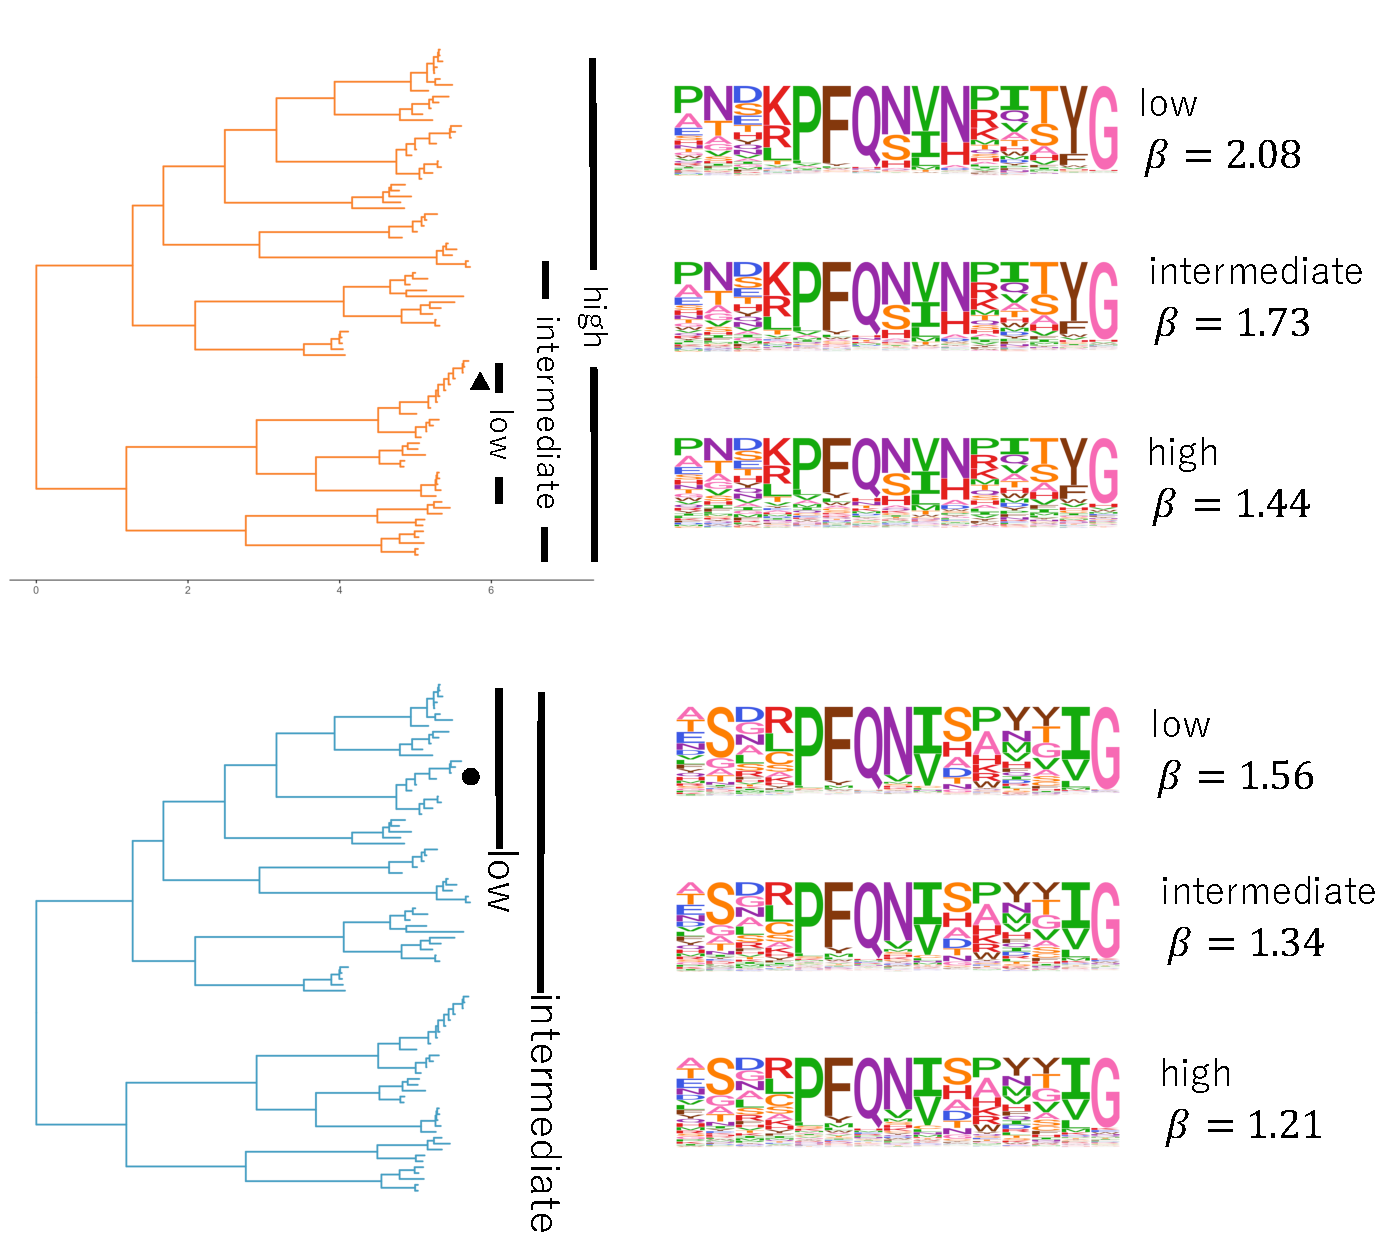
\includegraphics[width=0.85\textwidth]{figures/compete_4}}
\caption{\label{supp:compete_4}
}
\end{suppfig}


\clearpage 
\bibliographystyle{mbe}
\bibliography{references.bib}



\end{document}